% DPF 09 talk on strangeness in nucleon

\documentclass[10pt]{beamer}
\usefonttheme{professionalfonts} % using non standard fonts for beamer
\usefonttheme{serif} % default family is serif
\usepackage{amsmath}
\usepackage{mathtools}
%\documentclass[12pt]{beamerthemeSam.sty}
\usepackage{epsf}
%\usepackage{pstricks}
%\usepackage[orientation=portrait,size=A4]{beamerposter}
\geometry{paperwidth=160mm,paperheight=120mm}
%DT favorite definitions
\def\LL{\left\langle}	% left angle bracket
\def\RR{\right\rangle}	% right angle bracket
\def\LP{\left(}		% left parenthesis
\def\RP{\right)}	% right parenthesis
\def\LB{\left\{}	% left curly bracket
\def\RB{\right\}}	% right curly bracket
\def\PAR#1#2{ {{\partial #1}\over{\partial #2}} }
\def\PARTWO#1#2{ {{\partial^2 #1}\over{\partial #2}^2} }
\def\PARTWOMIX#1#2#3{ {{\partial^2 #1}\over{\partial #2 \partial #3}} }

\def\rightpartial{{\overrightarrow\partial}}
\def\leftpartial{{\overleftarrow\partial}}
\def\diffpartial{\buildrel\leftrightarrow\over\partial}

\def\BI{\begin{itemize}}
\def\EI{\end{itemize}}
\def\BE{\begin{displaymath}}
\def\EE{\end{displaymath}}
\def\BEA{\begin{eqnarray*}}
\def\EEA{\end{eqnarray*}}
\def\BNEA{\begin{eqnarray}}
\def\ENEA{\end{eqnarray}}
\def\EL{\nonumber\\}


\newcommand{\map}[1]{\frame{\frametitle{\textbf{Course map}}
\centerline{\includegraphics[height=0.86\paperheight]{../../map/#1.png}}}}
\newcommand{\wmap}[1]{\frame{\frametitle{\textbf{Course map}}
\centerline{\includegraphics[width=0.96\paperwidth]{../../map/#1.png}}}}

\newcommand{\etal}{{\it et al.}}
\newcommand{\gbeta}{6/g^2}
\newcommand{\la}[1]{\label{#1}}
\newcommand{\ie}{{\em i.e.\ }}
\newcommand{\eg}{{\em e.\,g.\ }}
\newcommand{\cf}{cf.\ }
\newcommand{\etc}{etc.\ }
\newcommand{\atantwo}{{\rm atan2}}
\newcommand{\Tr}{{\rm Tr}}
\newcommand{\dt}{\Delta t}
\newcommand{\op}{{\cal O}}
\newcommand{\msbar}{{\overline{\rm MS}}}
\def\chpt{\raise0.4ex\hbox{$\chi$}PT}
\def\schpt{S\raise0.4ex\hbox{$\chi$}PT}
\def\MeV{{\rm Me\!V}}
\def\GeV{{\rm Ge\!V}}

%AB: my color definitions
%\definecolor{mygarnet}{rgb}{0.445,0.184,0.215}
%\definecolor{mygold}{rgb}{0.848,0.848,0.098}
%\definecolor{myg2g}{rgb}{0.647,0.316,0.157}
\definecolor{abtitlecolor}{rgb}{0.0,0.255,0.494}
\definecolor{absecondarycolor}{rgb}{0.0,0.416,0.804}
\definecolor{abprimarycolor}{rgb}{1.0,0.686,0.0}
\definecolor{Red}           {cmyk}{0,1,1,0}
\definecolor{Grey}           {cmyk}{.7,.7,.7,0}
\definecolor{Lg}           {cmyk}{.4,.4,.4,0}
\definecolor{Blue}          {cmyk}{1,1,0,0}
\definecolor{Green}         {cmyk}{1,0,1,0}
\definecolor{Brown}         {cmyk}{0,0.81,1,0.60}
\definecolor{Black}         {cmyk}{0,0,0,1}

\usetheme{Madrid}


%AB: redefinition of beamer colors
%\setbeamercolor{palette tertiary}{fg=white,bg=mygarnet}
%\setbeamercolor{palette secondary}{fg=white,bg=myg2g}
%\setbeamercolor{palette primary}{fg=black,bg=mygold}
\setbeamercolor{title}{fg=abtitlecolor}
\setbeamercolor{frametitle}{fg=abtitlecolor}
\setbeamercolor{palette tertiary}{fg=white,bg=abtitlecolor}
\setbeamercolor{palette secondary}{fg=white,bg=absecondarycolor}
\setbeamercolor{palette primary}{fg=black,bg=abprimarycolor}
\setbeamercolor{structure}{fg=abtitlecolor}

\setbeamerfont{section in toc}{series=\bfseries}

%AB: remove navigation icons
\beamertemplatenavigationsymbolsempty
\title[Work and potential energy -- problem solving]{
  \textbf {Energy methods -- problem solving}\\
%\centerline{}
%\centering
%\vspace{-0.0in}
%\includegraphics[width=0.3\textwidth]{propvalues_0093.pdf}
%\vspace{-0.3in}\\
%\label{intrograph}
}

\author[W. Freeman] {Physics 211\\Syracuse University, Physics 211 Spring 2017\\Walter Freeman}

\date{\today}

\begin{document}

\frame{\titlepage}

\frame{\frametitle{\textbf{Announcements}}
\BI
\item{Office hours today: 5:10-6:50 -- probably me + coaches}
\item{Office hours moved from Friday to Thursday (5-7) to accommodate homework due date}
\item{Homework due Friday}
\item ODS students: exam 2 will be returned tomorrow in recitation (sorry for the delay)
\item Physics practice tomorrow will be an all-purpose help session: 7:30-9:30
\EI
}

\frame{\frametitle{\textbf{Where we've been, where we're going}}
  \BI
  \large
\item{Last time: we saw that ``potential energy'' is both a statement about nature and a bookkeeping trick to keep track of work}
\BI
\item{Potential energy only applies to conservative forces (gravity, springs)}
\item{Lets us account for the work done by these forces with no integrals required}
\item{Potential energy due to Earth's gravity: $U_g = mgy$}
\item{Potential energy in a spring: $U_e = \frac{1}{2}k(\Delta x)^2$}
\EI
\EI
}

\frame{\frametitle{\textbf{Power: rate of doing work}}
\large
A bit of mathematics that will be useful to you:

\bigskip

{\bf ``An object moves at a constant speed $\vec v$, subject to some force $\vec F$; at what rate does that force do work on the object?''}

\bigskip

An example: an airplane flies at v=1000 m/s, and its engines exert F=300 kN of thrust. What is the rate at which the engines do work (power)?

\bigskip

\centerline{Work = force $\cdot$ distance}
\pause
\centerline{Power = work / time}
\pause
\centerline{Power = force $\cdot$ distance / time}
\pause
\centerline{Power = force $\cdot$ (distance / time)}
\pause
\centerline{Power = force $\cdot$ velocity}
\pause
\centerline{$P = \vec F \cdot \vec v = {\color{Red}300 MW}$}

\bigskip

\BI
\item{The engines output 300 MW of power: this is around 10 liters per second of fuel even at 100\% efficiency!}
  \item{Some of that 300 MW of energy dissipated by drag heats up the airplane... (real numbers for a SR-71 Blackbird)}
    \EI
  }

\frame{\frametitle{\textbf{Problem-solving guide for problems involving energy}}
\large
\BI
\item Identify the various parts of the motion and what you need to know about them
\BI
\item Collisions/explosions: use conservation of momentum
\item Motion where you care only about begin/end states and not time: use work/energy methods
\item ``Where does it land'' projectile motion problems: can {\color{Red}not} use energy methods
\EI
\item Draw a series of snapshots, showing what your ``before'' and ``after'' pictures look like 
(you may have more than two in some problems)
\item Use force diagrams to calculate any forces you need to know
\item Application of the work-energy theorem:
\EI
$$KE_{\rm initial} + W_{\rm all} = KE_{\rm final}$$

\centerline{OR}

$$KE_{\rm initial} + PE_{\rm initial} + W_{\rm other} = KE_{\rm final} + PE_{\rm final}$$
}


\frame{\frametitle{\textbf{Sample problems}}

\Large
A mass $m$ is hung from a spring of spring constant $k$ and released. Which equation 
would let me find the distance $d$ that it falls before it comes back up?


\BI
\item A: $mgd - \frac{1}{2}kd^2 = 0$
\item B: $\frac{1}{2}kx^2 = mgd + \frac{1}{2}mv^2$
\item C: $0 = -mgd + \frac{1}{2}kd^2$
\item D: $mgd + \frac{1}{2}kd^2 = 0$
\EI
}

\frame{\frametitle{\textbf{Sample problems}}
\Large

A spring is used to launch a block up a ramp of total length L. The spring has spring constant $k$, the block has mass $m$,
the ramp is inclined an angle $\theta$, and it has a coefficient of kinetic friction $\mu_k$. 
I compress the spring a distance $x$ and let it go. How fast will the block be traveling when it reaches 
the top of the ramp?

\bigskip

Which equation would let me solve for this?

\BI
\item A: $\frac{1}{2}kx^2 + \mu mgL \cos \theta = \frac{mgL}{\sin \theta} - \frac{1}{2}mv_f^2$
\item B: $-\frac{1}{2}kx^2 + \mu mgL \sin \theta = \frac{mgL}{\sin \theta} + \frac{1}{2}mv_f^2$
\item C: $\frac{1}{2}kx^2 - \mu mgL \sin \theta = mgL \cos \theta + \frac{1}{2}mv_f^2$
\item D: $\frac{1}{2}kx^2 - \mu mgL \cos \theta = mgL \sin \theta + \frac{1}{2}mv_f^2$
\EI
}

\frame{\frametitle{\textbf{Sample problems}}
\Large
A car coasts down a ramp and then up around a loop of radius $r$. How high must the ramp be for the car
to make it around the loop? (See picture on document camera.)

\bigskip

How am I going to do this problem?

\large
\BI
\item A: Use conservation of momentum to relate the height of the ramp to the speed at the top of the loop,
then use kinematics to determine if it will fall or not.
\item B: Use conservation of energy to relate the height of the ramp to the speed at the top, then
use kinematics to determine at what point it will fall in the loop.
\item C: Use conservation of energy to relate the height of the ramp to the speed at the top, then
use Newton's second law and our knowledge of rotational motion to determine the required speed.
\item D: Use kinematics to relate the height of the ramp to the speed entering the loop, then
use Newton's second law and our knowledge of rotational motion to determine the required speed.
\EI
}


  \frame{\frametitle{\textbf{Sample problems}}
    \Large
  A truck pulling a heavy load with mass $m=4000$ kg wants to drive up a hill at a $30^\circ$ grade.

  \bigskip
  \bigskip

  If the truck's engine can produce 100 kW of power (134 hp), how fast can the truck go? (Neglect drag.)

}

\frame{\frametitle{\textbf{Sample problems}}
    \Large
A 1000 kg car has an engine that produces up to P=100 kW of power. If it accelerates as hard as it can, at what speed
does its acceleration become limited by the engine? 

\bigskip
\bigskip
\pause

(What else would limit its acceleration?)

\bigskip
\bigskip
\pause

At low speeds: static friction limits acceleration\\
At high speeds: engine power limits acceleration}



\frame{\frametitle{\textbf{Sample problems}}
  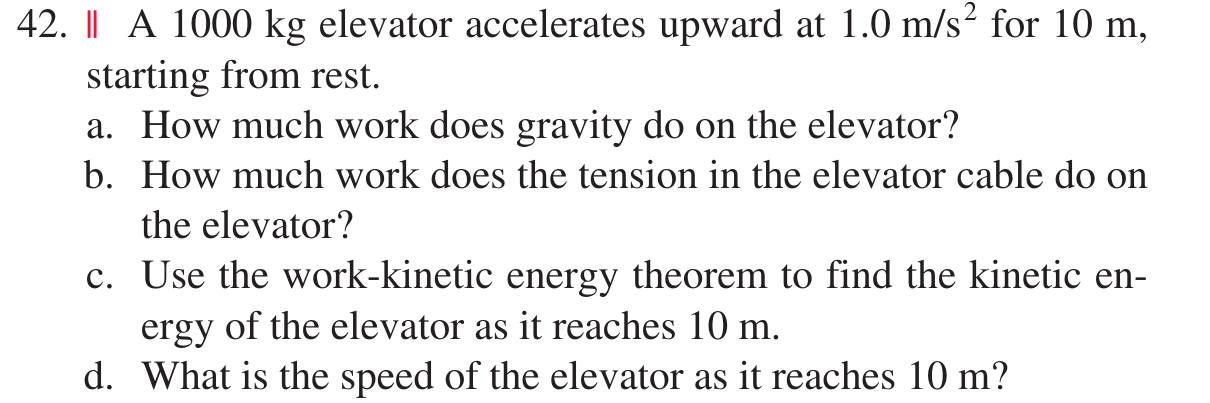
\includegraphics[width=0.7\textwidth]{elevator.png}
}




\frame{\frametitle{\textbf{Sample problems}}
  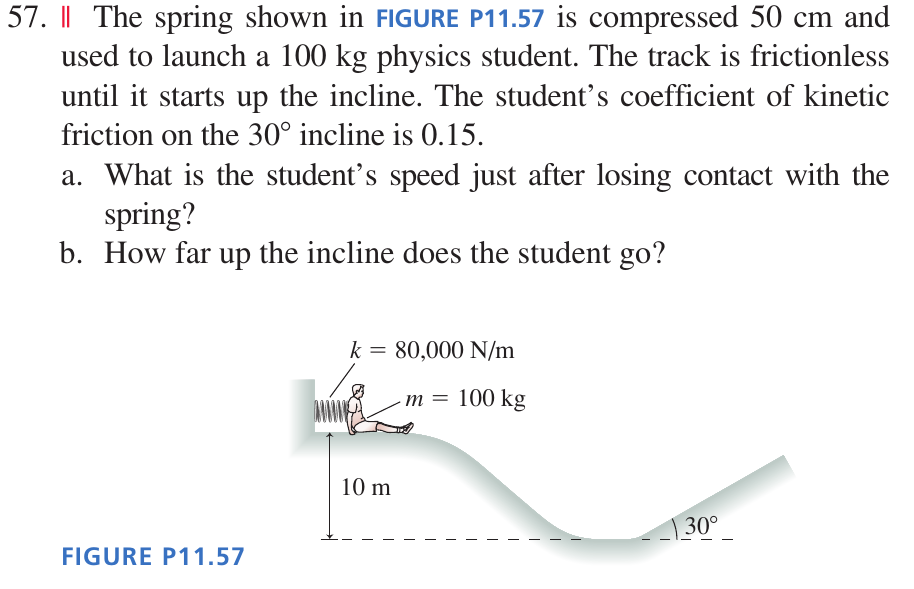
\includegraphics[width=0.7\textwidth]{student-on-spring.png}
}

\frame{\frametitle{\textbf{Sample problems}}
  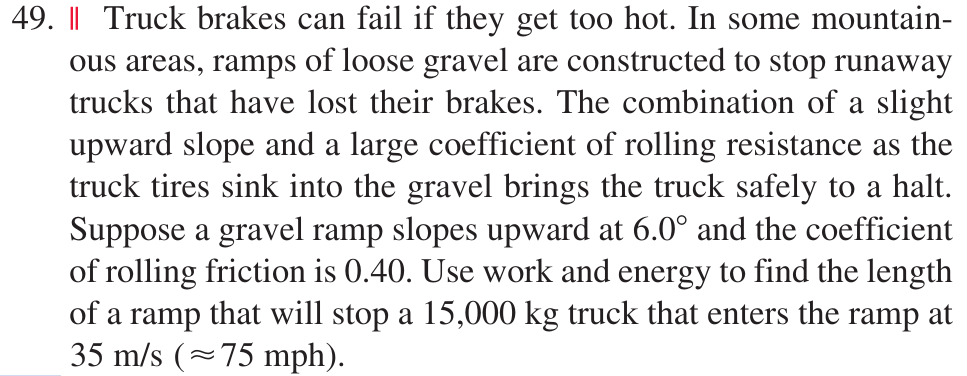
\includegraphics[width=0.7\textwidth]{runaway.png}
}





\end{document}
